\documentclass[11pt, aspectratio=169, compress]{beamer}
\usetheme[progressbar=frame title, numbering=fraction, sectionpage=none]{metropolis}      % Use metropolis theme 
\setbeamertemplate{section in toc}[sections numbered]
\setbeamertemplate{subsection in toc}[subsections numbered]
\useoutertheme[subsection=false]{miniframes}
\setbeamercolor{section in head/foot}{fg=white, bg=mDarkTeal}
\setbeamercolor{background canvas}{bg=white}
\setbeamerfont{section in head/foot}{series=\bfseries}

\usefonttheme[onlymath]{serif}
\usepackage{amsmath}
\usepackage{mathtools}
\usepackage{remreset}
\usepackage{ragged2e}
\usepackage{booktabs}
\usepackage{makecell}
\usepackage{listings}
\newcommand\setItemnumber[1]{\setcounter{enumi}{\numexpr#1-1\relax}}
\usepackage[utf8]{inputenc}
\usepackage[autostyle, english = american]{csquotes}
\MakeOuterQuote{"}
\usepackage{tikz}
\usetikzlibrary{arrows}
\usepackage{pgfplots}
\usetikzlibrary{positioning,decorations.text,calc,arrows.meta}
\usepackage[flushleft]{threeparttable}	% 3 part table 
\usepackage[justification=centering]{caption}
\captionsetup{skip=0pt}
\graphicspath{{C:/Users/ifyou/Documents/RA Jobs/LAMBDA/econometria-avanzada/lectures/01-RCT/fig}}

\makeatletter
\let\beamer@writeslidentry@miniframeson=\beamer@writeslidentry
\def\beamer@writeslidentry@miniframesoff{%
	\expandafter\beamer@ifempty\expandafter{\beamer@framestartpage}{}% does not happen normally
	{%else
		% removed \addtocontents commands
		\clearpage\beamer@notesactions%
	}
}
\newcommand*{\miniframeson}{\let\beamer@writeslidentry=\beamer@writeslidentry@miniframeson}
\newcommand*{\miniframesoff}{\let\beamer@writeslidentry=\beamer@writeslidentry@miniframesoff}
\beamer@compresstrue
\makeatother

%% Fonts
\usepackage{fontawesome}
\setfontfamily{\FA}{[FontAwesome.otf]}

%==============================================================
% Title Page
%==============================================================
%Information to be included in the title page:
\title{Introducción a RCT}
\author{Rony Rodrigo Maximiliano Rodriguez-Ramirez} 
\institute{maximiliano.rod.ra@gmail.com \\ DECRG | The World Bank}
\titlegraphic{\hfill
\includegraphics[height=1.5cm]{fig/dime.png}}
\date{\today}
%==============================================================
\begin{document}
	
\begin{frame}[plain]
	\maketitle  
\end{frame}

%\begin{frame}{Outline}
%\tableofcontents[hideallsubsections]
%\end{frame}
%------------------------------------------------

\begin{frame}[t]{Clean-up, Introducción}

Mi persona:
\begin{itemize}
  \item Mi nombre: Rony Rodrigo Maximilian Rodriguez Ramirez
  \item Mis cursos: R for Stata users, Stata Avanzado, Econometría Avanzada.
  \item Ubicación: Washington DC, The World Bank
  \item Projectos Actuales: Contraceptives in Cameroon (con Berk Özler y Susan Athey), Ukraine Tutoring Programs (Lelys Dinarte).
\end{itemize}

Datos sobre este curso:
\begin{itemize}
  \item \href{https://github.com/lambda-stata/econometria-avanzada}{Repositorio GitHub de este curso} \, \faGithub 
  \item Tipo de sessión: 45-50 minutes, 10 minutes descanso. De 3pm a 7pm Hora Perú.
\end{itemize}

\end{frame}

%------------------------------------------------
\section{Inferencia causal}
%------------------------------------------------
\subsection{Inferencia causal}
%------------------------------------------------
\begin{frame}{Poema de Robert Frost: The road not taken}
Two roads diverged in a yellow wood, \\
And sorry I could not travel both\\
And be one traveler, long I stood\\
And looked down one as far as I could\\
To where it bent in the undergrowth; 


Two roads diverged in a wood, and I--\\
I took the one less traveled by \\
And that has made all the difference. 

\end{frame}
%------------------------------------------------
\begin{frame}{Poema de Robert Frost: El camino no tomado}
Dos caminos se abrían en un bosque amarillo	\\
y lamentando no poder tomar ambos		\\
y siendo un sólo viajero, me quedé parado largo rato	\\
y en uno miré tan lejos como pude	\\
hasta dónde doblaba en la maleza;


Dos caminos se abrían en un bosque, y yo-- \\ 
tomé uno de ellos el menos transitado \\ 
y eso ha hecho toda la diferencia	
	
\end{frame}
%------------------------------------------------
\begin{frame}{Inferencia Causal}
El lenguaje de causa y efecto se usa todos los días en muchos
contextos, pero significa algo muy específico en la evaluación de impacto.

\begin{itemize}
\item Podemos pensar en la causalidad como: 
\begin{itemize}
	\item El efecto singular de un programa sobre un resultado de interés.
	\item Independiente de cualquier otro factor que intervenga.
\end{itemize}
\end{itemize}
\end{frame}
%------------------------------------------------
\begin{frame}{Inferencia Causal}
Por lo tanto, \textit{impacto} es definido como la comparación entre:
\begin{itemize}
	\item El resultado algún tiempo después de que se haya introducido el programa.
	\item El resultado en ese mismo momento si el programa no se hubiera introducido (El "\textit{contrafactural--counterfactual}"). 
\end{itemize}
\end{frame}
%------------------------------------------------
\section{Counterfactual}
%------------------------------------------------
\subsection{Counterfactual}
%------------------------------------------------
\begin{frame}{¿Cuál es el impacto?}
\begin{center}
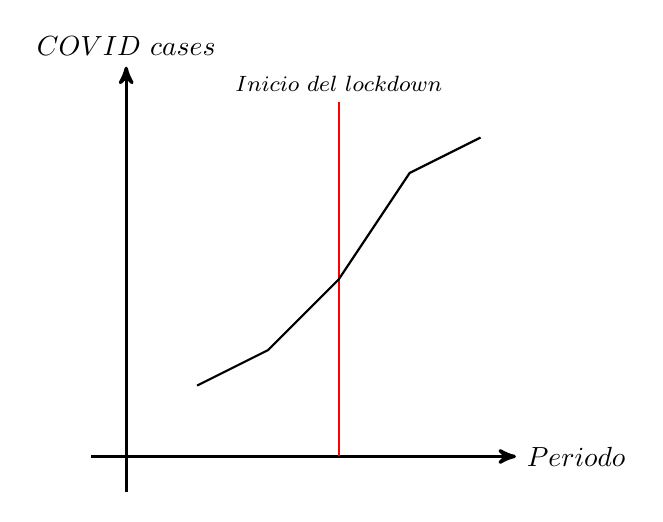
\begin{tikzpicture}[
	scale=4.5,
	axis/.style={very thick, ->, >=stealth'},
	important line/.style={thick},
	dashed line/.style={dashed, thin},
	pile/.style={thick, ->, >=stealth', shorten <=2pt, shorten
		>=2pt},
	every node/.style={color=black}
	]
	% axis
	\draw[axis] (-0.1,0)  -- (1.1,0) node(xline)[right]
	{$Periodo$};
	\draw[axis] (0,-0.1) -- (0,1.1) node(yline)[above] 
	{$COVID~cases$};
	\draw[red, important line] (0.6,0) -- (0.6, 1) node(time)[above] 
	{\footnotesize $Inicio~del~lockdown$}; 
	% Lines
	\draw[important line] (0.2, 0.2) -- (0.4, 0.3) -- (0.6, 0.5) -- (0.8,0.8) -- (1, 0.9);
\end{tikzpicture}
\end{center}
\end{frame}

%------------------------------------------------
\begin{frame}{¿Cuál es el impacto?}
\begin{center}
	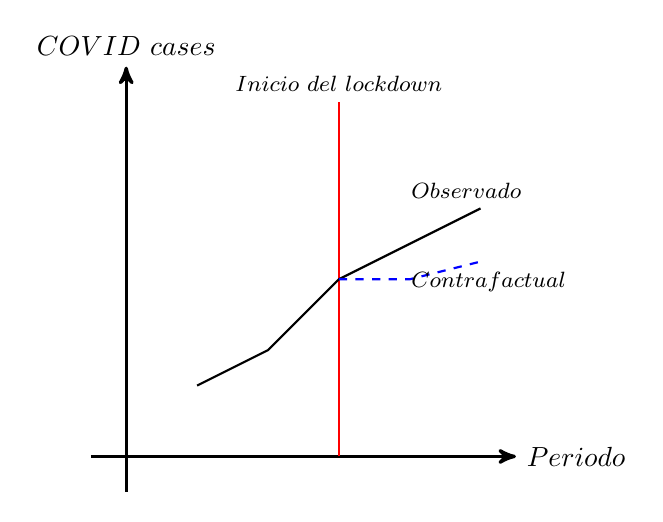
\begin{tikzpicture}[
	scale=4.5,
	axis/.style={very thick, ->, >=stealth'},
	important line/.style={thick},
	dashed line/.style={dashed, thin},
	pile/.style={thick, ->, >=stealth', shorten <=2pt, shorten
		>=2pt},
	every node/.style={color=black}
	]
	% axis
	\draw[axis] (-0.1,0)  -- (1.1,0) node(xline)[right]
	{$Periodo$};
	\draw[axis] (0,-0.1) -- (0,1.1) node(yline)[above] 
	{$COVID~cases$};
	\draw[red, important line] (0.6,0) -- (0.6, 1) node(time)[above] 
	{\footnotesize $Inicio~del~lockdown$}; 
	% Lines
	\draw[important line] (0.2, 0.2) -- (0.4, 0.3) -- (0.6, 0.5) -- (0.8,0.6) -- (1, 0.7)
	node[above, text width=5em] {\footnotesize $Observado$};
	\draw[blue, dashed, important line] (0.6, 0.5) -- (0.8,0.5) -- (1, 0.55)
	node[below, text width=5em] {\footnotesize $Contrafactual$}; 
	\end{tikzpicture}
\end{center}
\end{frame}
%------------------------------------------------
\begin{frame}{¿Cuál es el impacto?}
\begin{center}
	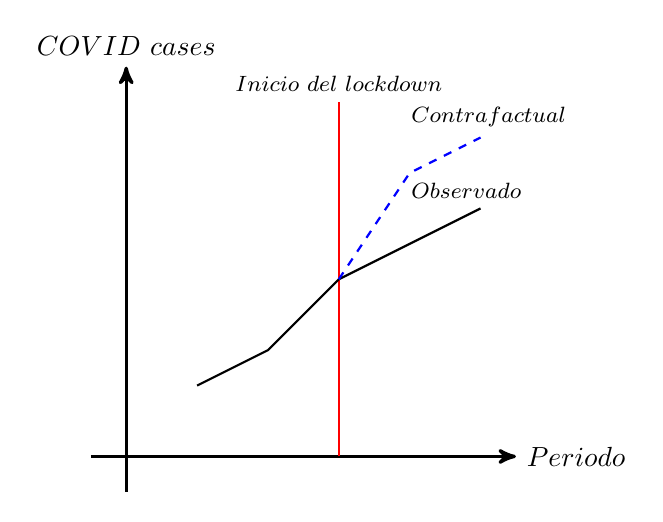
\begin{tikzpicture}[
	scale=4.5,
	axis/.style={very thick, ->, >=stealth'},
	important line/.style={thick},
	dashed line/.style={dashed, thin},
	pile/.style={thick, ->, >=stealth', shorten <=2pt, shorten
		>=2pt},
	every node/.style={color=black}
	]
	% axis
	\draw[axis] (-0.1,0)  -- (1.1,0) node(xline)[right]
	{$Periodo$};
	\draw[axis] (0,-0.1) -- (0,1.1) node(yline)[above] 
	{$COVID~cases$};
	\draw[red, important line] (0.6,0) -- (0.6, 1) node(time)[above] 
	{\footnotesize $Inicio~del~lockdown$}; 
	% Lines
	\draw[important line] (0.2, 0.2) -- (0.4, 0.3) -- (0.6, 0.5) -- (0.8,0.6) -- (1, 0.7)
	node[above, text width=5em] {\footnotesize $Observado$};
	\draw[blue, dashed, important line] (0.6, 0.5) -- (0.8,0.8) -- (1, 0.9)
	node[above, text width=5em] {\footnotesize $Contrafactual$}; 
	\end{tikzpicture}
\end{center}
\end{frame}
%------------------------------------------------
\begin{frame}{Contrafactual}
El \textit{contrafactual} representa el estado del mundo que los participantes del programa habrían experimentado en ausencia del programa (es decir, si no hubieran participado en el programa).

\textbf{Sin embargo:}
\begin{itemize}
	\item No podemos observar el contrafactual.
	\item Necesitamos `` crear '' el contrafactual.
\end{itemize}
\end{frame}
%------------------------------------------------
\begin{frame}{Un ejemplo}
  \begin{table}[H]
  \centering 
    \begin{threeparttable}
    \caption{Resultados y tratamientos para Inayat y Abdul}
    \small 
    \begin{tabular}{l c c} \hline \hline 
                              &LATIF, Abdul 	& ULLAH, Inayat \\ \hline
    Resultado potencial sin sesión de TA: $ Y_{0i} $	& 90	& 94  	\\
    Resultado potencial con la sesión de TA: $ Y_{1i}$ 	& 95	& 94  	\\
    Tratamiento (sesión de TA elegida):$ D_i $			& 1		& 0 	\\
    Resultado real de la clase: $ Y_{i} $				& 95	& 94   	\\ 
    Efecto del tratamiento: $ Y_{1i} - Y_{0i} $			& 5		& 0  	\\ \hline 
    \end{tabular}
    \end{threeparttable}
  \end{table}
\end{frame}
%------------------------------------------------
\begin{frame}{Un ejemplo}
\begin{itemize}
\item Si solo comparamos los resultados de Latif, tendríamos que el resultado es $ 5 $. 
\item Si solo comparamos los de Ullah, tendríamos que el resultado es $ 0 $.
\item Por lo tanto, ¿deberíamos comparar $ Y_{\mathrm{Latif}} - Y_{\mathrm{Ullah}} ? $
\end{itemize}

Necesitamos vincular los resultados observados y potenciales de la siguiente manera:
\begin{align*}
Y_{\mathrm{Latif}} - Y_{\mathrm{Ullah}} &= Y_{1,\mathrm{Latif}} - Y_{0,\mathrm{Ullah}} \\ 
&= \underbrace{Y_{1,\mathrm{Latif}} - Y_{0,\mathrm{Latif}}}_{5} + \underbrace{Y_{0,\mathrm{Latif}} - Y_{0,\mathrm{Ullah}}}_{-4}. \\ 
\end{align*}
La falta de comparabilidad capturada por el segundo término se llama \textit{\textbf{sesgo de selección--selection bias.}}
\end{frame}
%------------------------------------------------
\begin{frame}{Representación matemática}
\begin{align*}
E[Y_i | D=1] - E[Y_i | D_i=0] &= E[Y_{1i} | D_i=1] - E[Y_{0i} | D_i=0] \\
&= E[Y_{1i} | D_i=1] - E[Y_{0i} | D_i=1] \\
&+ E[Y_{0i} | D_i=1] - E[Y_{0i} | D=0] \\ 
&= \underbrace{E[Y_{1i} - Y_{0i} | D_i=1]}_{\text{Impacto}} +  \underbrace{E[Y_{0i} | D_i=1] - E[Y_{0i} | D=0]}_{\text{Sesgo de selección}}\\ 
\end{align*}
La contraparte de la regresión para obtener el impacto es:
\begin{equation}
Y_i = \alpha + \beta D_{i} + \epsilon_i 
\end{equation}
\end{frame}
%------------------------------------------------
\begin{frame}{RCT cont.}
	\begin{center}
		El objetivo de la mayoría de las investigaciones empíricas es superar el sesgo de selección y, por tanto, decir algo sobre el efecto causal de una variable como $D_i$. 
	\end{center}
\end{frame}
%------------------------------------------------
\begin{frame}{RCT cont.}
	La asignación aleatoria resuelve el problema del sesgo de selección: 
	\begin{itemize}
		\item $Y_{0i}, Y_{1i}$ son independientes de $D_i$; 
		\item En este contexto, tenemos que enfocarnos directamente en la asignación de $D_i$.
	\end{itemize}
\end{frame}
%------------------------------------------------
\section{Randomized Controlled Trials}
\subsection{Randomized Controlled Trials}
%------------------------------------------------
\begin{frame}{El RCT ideal}
	\begin{itemize}
	\item La idea central de un experimento aleatorio ideal es que el efecto causal se puede medir (1) seleccionando individuos al azar de una población y luego (2) administrando el tratamiento al azar a algunos de los individuos.
	\begin{itemize}
		\item ¿Es el muestreo aleatorio lo mismo que la asignación aleatoria?
	\end{itemize}
	\item Si el tratamiento se asigna al azar, entonces el nivel de tratamiento se distribuye independientemente de cualquiera de los otros determinantes del resultado, eliminando así la posibilidad de sesgo de variable omitida (OVB).
	\end{itemize}
\end{frame}
%------------------------------------------------
\begin{frame}{Amenazas a la validez interna}
	\textit{Validez Interna}: cuando las inferencias estadísticas sobre efectos causales son válidas para la población en estudio.
	
	Amenaza (1) -- No aleatorizar:
	\begin{itemize}
		\item La asignación aleatoria al grupo de tratamiento y control es la característica fundamental de un experimento controlado aleatorio que permite estimar el efecto causal.
		
		\item Si el tratamiento no se asigna al azar, sino que se basa en parte en las características o preferencias del sujeto, los resultados reflejarán tanto el efecto del tratamiento como el efecto de la asignación no aleatoria.
	\end{itemize}
\end{frame}
%------------------------------------------------
\begin{frame}{Amenazas a la validez interna}
	Amenaza (2) -- No seguir el protocolo de tratamiento:
	
	\begin{itemize}
		\item El hecho de que los individuos no sigan completamente el protocolo de tratamiento aleatorizado se denomina cumplimiento parcial del tratamiento.
		\item En un experimento de programa de capacitación laboral, algunos de los sujetos asignados al grupo de tratamiento podrían no presentarse a las sesiones de capacitación y, por lo tanto, no recibir el tratamiento. De manera similar, las personas del grupo de control podrían de alguna manera recibir la capacitación de todos modos.
	\end{itemize}
\end{frame}
%------------------------------------------------
\begin{frame}{Amenazas a la validez interna}
	Amenaza (3) -- Atrición selectiva:
	\begin{itemize}
		\item La deserción se refiere a los sujetos que abandonan el estudio después de haber sido asignados al azar al grupo de tratamiento o de control.
		\item Si el motivo de la deserción está relacionado con el tratamiento en sí, entonces la deserción da como resultado un sesgo en el estimador MCO del efecto causal.
		
		\begin{itemize}
			\item Si los aprendices más capaces abandonan el experimento del programa de capacitación laboral porque obtienen trabajos fuera de la ciudad, al final del experimento solo quedan los miembros menos capaces del grupo de tratamiento.
		\end{itemize}
	\end{itemize}
\end{frame}
%------------------------------------------------
\begin{frame}{Amenazas a la validez interna}
	Amenaza (4) -- Efectos experimentales (Howthorne effects): 
	\begin{itemize}
		\item En experimentos con sujetos humanos, el mero hecho de que los sujetos estén en un experimento puede cambiar su comportamiento.
		\item Protocolo "doble ciego": en un experimento con fármacos, fármaco real frente a placebo.
	\end{itemize}
\end{frame}
%------------------------------------------------
\begin{frame}{Amenazas a la validez externa}
	\textit{Validez externa}: cuando la inferencia y las conclusiones se pueden generalizar de la población y el entorno estudiado a otras poblaciones y entornos.
	
	Amenaza (1) -- Muestra no representativa: cuando la población estudiada y la población de interés no son suficientemente similares para justificar la generalización de los resultados experimentales.
	
	\begin{itemize}
		\item Si se evalúa un programa de capacitación laboral en un experimento con ex reclusos, es posible que los resultados no se generalicen a los trabajadores que nunca han cometido un delito.
		\item Si los participantes experimentales son voluntarios, entonces estos voluntarios podrían estar más motivados que la población en general y, para ellos, el tratamiento podría tener un efecto mayor.
	\end{itemize}
\end{frame}
%------------------------------------------------
\begin{frame}{Amenazas a la validez externa}
	Amenaza (2) -- Programa no representativo:
	
	\begin{itemize}
		\item El programa en un experimento de pequeña escala y estrictamente monitoreado podría ser bastante diferente al programa realmente implementado. 
		
		\item Si el programa realmente implementado está ampliamente disponible, es posible que el programa de ampliación no proporcione el mismo control de calidad que la versión experimental o que esté financiado a un nivel inferior.
	\end{itemize}
\end{frame}
%------------------------------------------------
\begin{frame}{Amenazas a la validez externa}
	Amenaza (3) -- Efectos de equilibrio general:
	
	\begin{itemize}
		\item Convertir un pequeño programa experimental temporal en un programa permanente y generalizado podría cambiar el entorno económico lo suficiente como para que los resultados del experimento no se puedan generalizar.
		\item Reducción del tamaño de las aulas: a gran escala, podría aumentar la demanda de profesores y cambiar el tipo de persona que se siente atraída por la docencia.
	\end{itemize}
\end{frame}
%------------------------------------------------
\begin{frame}{Diferentes métodos de aleatorización}
	\begin{itemize}
		\item (1) Sobresuscripción (Acceso al programa): Más común. 
		\begin{itemize}
			\item Si los recursos limitados son una carga para el programa, la implementación se puede asignar al azar a un subconjunto de participantes elegibles, y los sujetos elegibles restantes que no reciben el programa pueden considerarse controles.
		\end{itemize}	
		\item Ejemplo: 
		
		El programa de vales escolares PACS, establecido por el gobierno de Colombia a fines de 1991: estos vales cubrían aproximadamente la mitad de los gastos de escolarización de los estudiantes ingresantes y eran renovables según el desempeño de los estudiantes. (Angrist et al. 2002. Vales para la educación privada en Colombia. American Economic Review 92.5)
	\end{itemize}
\end{frame}
%------------------------------------------------
\begin{frame}{Diferentes métodos de aleatorización}
	\begin{itemize}
		\item (2) Incorporación paulatina aleatorizada (tiempo de acceso al programa): este enfoque incluye gradualmente el programa en un conjunto de áreas elegibles, de modo que los controles representan áreas elegibles que aún esperan recibir el programa. Este método ayuda a aliviar los problemas de equidad. Pero, efectos anticipatorios y sin efectos a largo plazo.	
		\item Ejemplo: 
		
		PROGRESA (ahora llamado Oportunidades) se dirigió a los pobres extremos en México. Un tercio de las comunidades elegibles seleccionadas al azar sufrieron un retraso de 18 meses en su ingreso al programa, y los dos tercios restantes recibieron el programa al inicio.
	\end{itemize}
\end{frame}
%------------------------------------------------
\begin{frame}{Diferentes métodos de aleatorización}
	\begin{itemize}
		\item (3) Diseño de estímulo: en lugar de aleatorizar el tratamiento, los investigadores asignan aleatoriamente a los sujetos un anuncio o incentivo para participar en el programa.
	\end{itemize}
\end{frame}
%------------------------------------------------
\begin{frame}{Niveles de randomización}
	\begin{itemize}
		\item \textit{Derrame}: para reducir el riesgo de derrame, la aleatorización se lleva a cabo a nivel del hogar o la escuela.
		\item \textit{Resentimiento}: es menos probable que cooperen con la recopilación de datos cuando ven que otros reciben beneficios mientras ellos no reciben nada, por lo que podría ayudar a reducir el desgaste
		\item Poder estadístico y nivel de aleatorización: compensación
	\end{itemize}
\end{frame}
%------------------------------------------------
\begin{frame}{Heterogeneidad en los impactos}
	Efecto promedio del tratamiento (ATE) versus efecto heterogéneo
	\begin{itemize}
		\item Análisis de interacción
		\item Análisis de subgrupos
		\item Ejemplos: nivel de ingresos, nivel de educación, para hogares cuyos hijos ya estaban matriculados
		en la escuela, Para niñas que todavía estaban matriculadas en la escuela, etc.
    \item Más ejemplos sobre esto más adelante.
	\end{itemize}
\end{frame}
%------------------------------------------------
\begin{frame}{Valor de una encuesta de referencia: Baseline survey}
	\begin{itemize}
		\item \textbf{Balance de aleatorización:} 
					
		Las encuestas de línea de base permiten verificar que la aleatorización se realizó de manera adecuada.
		
		\item \textbf{Análisis de heterogeneidad:} 
				
		Las encuestas de línea de base permiten examinar las interacciones entre las condiciones iniciales y el impacto del programa.
	\end{itemize}
\end{frame}
%------------------------------------------------
\section{Más sobre efectos y sesgos}
\subsection{Más sobre efectos y sesgos}
%------------------------------------------------
\begin{frame}{Recap: sobre las fuentes del sesgo}
	\begin{itemize}
		\item \textit{Externalidades}: ocurre cuando las personas no tratadas se ven afectadas por el tratamiento.
		\item \textit{Atrición}: ocurre cuando algunos individuos tratados abandonan la muestra original.
		\item \textit{Efectos Hawthorne y John Henry}: ocurre cuando la propia evaluación puede provocar que el grupo de tratamiento o de control cambie su comportamiento.
	\end{itemize}
\end{frame}
%------------------------------------------------
\begin{frame}{En términos de estimación}
	\begin{itemize}
		\item Las externalidades llevarán a una subestimación (sobreestimación) del efecto del tratamiento si son positivas (negativas).
		\item Algunas técnicas pueden utilizarse para estimar la magnitud de las externalidades y, por lo tanto, neutralizar el sesgo que inducen.
		\item Por ejemplo, al evaluar el impacto de las sesiones de asistencia técnica en los puntajes de las pruebas, uno puede preocuparse por las externalidades de la información: 
		\begin{itemize}
			\item los estudiantes del grupo de tratamiento pueden hablar con los del grupo de control sobre los contenidos de las sesiones de asistencia técnica.
		\end{itemize}
	\end{itemize}
\end{frame}
%------------------------------------------------
\begin{frame}{Externalidades}
	\begin{itemize}
		\item La primera técnica para abordar el problema es aprovechar la variación en la exposición entre grupos que surge naturalmente de la aleatorización.
		\item Por ejemplo, preguntando a los estudiantes tanto del grupo de tratamiento como del grupo de control el nombre de los 3 estudiantes con los que discuten los materiales del curso con más frecuencia (a continuación, nos referiremos a ellos como "amigos").
	\end{itemize}
\end{frame}
%------------------------------------------------
\begin{frame}{Externalidades}
	\begin{itemize}
		\item Para tener una idea de la magnitud de los \textit{derrames} de información, se puede comparar:
		\begin{itemize}
			\item las puntuaciones de las pruebas de los amigos del grupo de tratamiento en el grupo de control.
			\item las puntuaciones de las pruebas de los amigos del grupo de control en el grupo de control.
		\end{itemize}
	\end{itemize}
\end{frame}
%------------------------------------------------
\begin{frame}{Externalidades}
	\begin{itemize}
		\item La segunda técnica consiste en variar deliberadamente el nivel de exposición a un tratamiento dentro de un grupo.
		
		\item Por ejemplo, en el estudio de información y participación 401 (k) (es decir, cuentas de impuestos diferidos), Duflo y Saez (2003) aleatorizaron la oferta de obtener un incentivo para asistir a la sesión de información en dos niveles.
	\end{itemize}
\end{frame}
%------------------------------------------------
\begin{frame}{Externalidades}
	\begin{itemize}
		\item Primero se eligió al azar un conjunto de departamentos universitarios para recibir tratamiento, y luego se ofrecieron incentivos económicos a un conjunto aleatorio de individuos dentro de los departamentos de tratamiento.
		
		\item Esto permitió a los autores explorar tanto el efecto directo sobre la asistencia y la inscripción al plan de recibir un incentivo como el efecto indirecto de estar en un departamento en el que se habían ofrecido incentivos a otros.
	\end{itemize}
\end{frame}
%------------------------------------------------
\begin{frame}{Atrición}
	\begin{itemize}
		\item La deserción no causará un sesgo si es aleatorio (aún reduce el poder estadístico), sin embargo, inducirá un sesgo tan pronto como se correlacione con el impacto que el tratamiento tiene en cada individuo.
		\item Por ejemplo, surgirá un sesgo si aquellos que se benefician menos de las sesiones de asistencia técnica tienden a abandonar la muestra. 
		\item Por lo tanto, la gestión del desgaste durante el proceso de recopilación de datos es esencial.
	\end{itemize}
\end{frame}
%------------------------------------------------
\begin{frame}{Atrición}
	\begin{itemize}
		\item Más precisamente, esto requiere recopilar buena información en un cuestionario de referencia sobre cómo encontrar a cada individuo nuevamente, en caso de que decida dejar el grupo después del tratamiento (preguntando, por ejemplo, los nombres de los familiares que pueden ser entrevistados si no se puede encontrar al encuestado durante la encuesta postratamiento).
		\item Por supuesto, el seguimiento de TODOS los atridores suele ser demasiado caro, pero el seguimiento con solo una muestra aleatoria de los atridores es una buena alternativa.
	\end{itemize}
\end{frame}
%------------------------------------------------
\begin{frame}{HJH effects}
	\begin{itemize}
		\item \textit{\textbf{Efecto Hawthorne (el efecto del observador)}}: los individuos del grupo de tratamiento, debido a que son conscientes de ser observados, pueden alterar su comportamiento durante el experimento (en comparación con lo que suele ser) para complacer al experimentador (por ejemplo, los estudiantes que tienen la oportunidad tomar sesiones de asistencia técnica también puede decidir trabajar más duro).
	\end{itemize}
\end{frame}
%------------------------------------------------
\begin{frame}{HJH effects}
	\begin{itemize}
		\item \textit{\textbf{Efecto John Henry}}: los individuos en el grupo de control, en caso de que sean conscientes de ser un grupo de control, pueden sentirse ofendidos al obtener este estado experimental y, por lo tanto, podrían reaccionar alterando también su comportamiento (por ejemplo, los estudiantes que no tienen la oportunidad de tomar TA sesiones pueden decidir trabajar más duro o relajarse).
	\end{itemize}
\end{frame}
%------------------------------------------------
\begin{frame}{HJH effects}
	\begin{itemize}
		\item Una forma de eliminar los efectos de HJH es continuar monitoreando el impacto de una intervención, una vez finalizado el experimento oficial.
		
		\item El hecho de que el impacto medido sea similar cuando el programa ya no está siendo evaluado oficialmente y cuando el programa es evaluado oficialmente significa que no se debe a los efectos HJH.
	\end{itemize}
\end{frame}
%------------------------------------------------
\begin{frame}{HJH effects}
	\begin{itemize}
		\item Si no son similares, la estimación del efecto del tratamiento debe basarse en la encuesta "postratamiento".
		
		\item Las evaluaciones también pueden diseñarse para ayudar a desenredar los diversos canales y ayudar a mejorar las preocupaciones sobre los efectos de HJH.
	\end{itemize}
\end{frame}
%------------------------------------------------
\section{Treatment effects}
\subsection{Treatment effects}
%------------------------------------------------
\begin{frame}{Incumplimiento}
	\begin{table}[H]
		\centering 
		\begin{threeparttable}
			\centering 
			\small 
			\begin{tabular}{l c c} \hline \hline 
									& Asignación a tratamiento	& Asignación a control 	\\ \hline
				Cumplidores			& Tratado 					& Control 				\\
				Siempre tomadores 	& Tratado					& Tratado				\\
				Nunca tomadores		& No tratado				& No tratado			\\
				Desafiantes			& No tratado 				& Tratado				\\ \hline 
			\end{tabular}
		\end{threeparttable}
	\end{table}
\end{frame}
%------------------------------------------------
\begin{frame}{Incumplimiento}
	\begin{table}[H]
		\centering 
		\begin{threeparttable}
			\centering 
			\small 
			\begin{tabular}{l c c} \hline \hline 
									& Asignación a tratamiento	& Asignación a control 		\\ 
									& resultado promedio = 50	& resultado promedio = 10 	\\ \hline
				Cumplidores			& 0 				& 0 				\\
				Siempre tomadores 	& 10				& 10				\\
				Nunca tomadores		& 80				& 80				\\
				Desafiantes			& 10 				& 10 				\\ \hline 
			\end{tabular}
		\end{threeparttable}
	\end{table}
\end{frame}
%------------------------------------------------
\begin{frame}{Incumplimiento}
  El cumplimiento imperfecto es cuando las personas no siguen su asignación de tratamiento. Mientras que los cumplidores son personas que son inducidas a aceptar el tratamiento solo porque fueron asignados para recibirlo (y no lo toman si no se les asigna un tratamiento), los incumplidores se componen de tres grupos:

  \begin{itemize}
    \item \textit{Siempre tomadores}: siempre toman el tratamiento incluso si están asignados al grupo de control

    \item \textit{Personas que nunca lo toman}: siempre rechacen el tratamiento, incluso si están asignados al grupo de tratamiento

    \item \textit{Desafiantes}: hacen lo contrario de su asignación de tratamiento
  \end{itemize}

\end{frame}
%------------------------------------------------
\begin{frame}{Incumplimiento}

  \begin{itemize}
  \item El incumplimiento puede ser unilateral o bilateral. 
  
    \begin{itemize}
      \item El incumplimiento unilateral es cuando las personas asignadas al grupo de tratamiento rechazan el tratamiento O las personas asignadas al grupo de control lo toman. 
    
      \item El incumplimiento bilateral es cuando ocurren ambos.
    \end{itemize}

  \end{itemize}

\end{frame}
%------------------------------------------------
\begin{frame}{Incumplimiento}

  \begin{itemize}
    \item En muchos casos, los investigadores y los formuladores de políticas se preocupan por identificar el impacto de la oferta del programa en la población a la que se le ofreció, incluso si algunos de ellos no lo aceptaron, ya que esto se parecerá a lo que probablemente suceda si el programa se despliega. 
  
    \item La intención de tratar (ITT) es una estimación del efecto del programa en las personas asignadas al tratamiento, independientemente de su aceptación. Es decir, el ITT se obtiene al hacer una regresión del resultado en la asignación de tratamiento para toda la muestra.
  \end{itemize}
\end{frame}
%------------------------------------------------
\begin{frame}{Incumplimiento}
  
  A menudo (aunque no siempre) proporcionará un límite inferior en el ATE, ya que incluye en el grupo de tratamiento a algunas personas que no recibieron el tratamiento (bajo el supuesto de que se habrían beneficiado menos del tratamiento que aquellos que lo aceptaron), y puede incluir en el grupo de comparación a algunas personas que de hecho recibieron el tratamiento.
  
\end{frame}
%------------------------------------------------
\begin{frame}{Varios efectos del tratamiento}
	\begin{itemize}
		\item Efecto promedio del tratamiento (ATE): el efecto esperado del tratamiento en una persona seleccionada al azar de la población: $E(Y_{i}^{T}-Y_{i}^{C})$. 
		\item Efecto por intención de tratar (ITT): ATE entre aquellos en el brazo de tratamiento (puede que no siempre cumplan con el tratamiento), $E(Y_{i}^{D} - Y_{i}^{C}| D)$, donde $D$ significa ser asignado al brazo de tratamiento.
		\item Tratamiento promedio en el tratado (ATT): ATE entre los que están siendo realmente tratados (en el brazo de tratamiento), $E(Y_{i}^{D} - Y_{i}^{C}| T)$, donde $T$ significa que están siendo tratados. Tenga en cuenta que tenemos $ T \subseteq D$.
	\end{itemize}
\end{frame}
%------------------------------------------------
\begin{frame}{Varios efectos del tratamiento}
	\begin{itemize}
		\item En RCT, si solo hay "cumplidores" en la muestra, tenemos $ATE = ITT = ATT = LATE$. 
		\item Bajo RCT, si solo hay "cumplidores" y "nunca tomadores" en la muestra, no podemos calcular ATE. ITT es la diferencia entre las medias de tratamiento y el grupo de control. Además, $ ATT = LATE = ITT/$share of compliers.
		\item Bajo RCT, si hay "cumplidores", "siempre tomadores" y "nunca tomadores" en la muestra, no podemos calcular ATE. ITT es la diferencia entre las medias de tratamiento y el grupo de control. Además, $ ATT \neq LATE = ITT/$share of compliers.
		\begin{itemize}
			\item Tenga en cuenta que es posible que los "siempre tomadores " no existan en algunos entornos experimentales, p. Ej., Subvenciones, introducción de nueva tecnología, etc.
		\end{itemize}
	\end{itemize}
\end{frame}
%------------------------------------------------
\begin{frame}{Clustering y errores estándar robustos}

  Independientemente de su procedimiento de muestreo o asignación, generalmente se recomienda utilizar siempre errores estándar robustos a la heterocedasticidad en su especificación de regresión: White (1980), Angrist \& Pischke (2009) y Wooldridge (2013).

  Según lo aconsejado por Abadie et al. (2017) y resumido por David McKenzie, hay dos razones por las que desearía agrupar sus errores estándar:
  
  \begin{itemize}
    \item Cuando haya asignado un tratamiento en otra unidad que no sea aquella en la que está midiendo los resultados.
    \item Cuando haya muestreado unidades de una población mediante muestreo por conglomerados.
  \end{itemize}

\end{frame}
%------------------------------------------------
\begin{frame}{Clustering y errores estándar robustos}

  \begin{enumerate}
    \item \textbf{Cuando haya asignado un tratamiento en otra unidad que no sea aquella en la que está midiendo los resultados.}
    
    Aquí, Abadie et al. (2017) recomiendan la agrupación en el nivel en el que se asignó el tratamiento. Por ejemplo, si se asigna el tratamiento a nivel de aldea pero se miden los resultados a nivel individual, los errores estándar deberían agruparse a nivel de aldea. 
    
    Tenga en cuenta que incluso sin una asignación aleatoria agrupada, si tiene observaciones repetidas de la misma unidad (por ejemplo, si tiene datos de panel), querrá agrupar los errores estándar por unidad para tener en cuenta las correlaciones dentro de la unidad a lo largo del tiempo.
 
  \end{enumerate}
\end{frame}
%------------------------------------------------
\begin{frame}{Clustering y errores estándar robustos}

  \begin{enumerate}
    \setItemnumber{2}
    \item \textbf{Cuando haya muestreado unidades de una población mediante muestreo por conglomerados.}
    
    Las consideraciones clave aquí son cómo se seleccionó la muestra, si hay conglomerados en la población de interés que no están en la muestra y si desea decir algo sobre la población de la cual se extrajo la muestra. También es posible que desee utilizar ponderaciones de muestra para generalizar los resultados a la población; ver más abajo.
  \end{enumerate}
\end{frame}
%------------------------------------------------
\section{Ética}
\subsection{Ética}

\begin{frame}{Ética}
  Si está realizando un RCT, incluya una subsección sobre consideraciones éticas:

  \begin{itemize}
    \item Incluya una oración para la recopilación de datos de rutina, cuestiones de consentimiento informado;

    \item Proporcione los números de aprobación del IRB, pero también proporcione un enlace a un documento que contenga sus protocolos de estudio detallados (posiblemente su presentación al IRB) o inclúyalo en un apéndice; y
    
    \item Discutir en detalle cuestiones éticas más espinosas que se han cubierto en los protocolos del estudio, proporcionar una evaluación de los riesgos, compararlos con puntos de referencia razonables, dar una sensación de equilibrio y la importancia del estudio para proporcionar beneficios mediante la generación de nuevos conocimientos.
  \end{itemize}
  
\end{frame}
%------------------------------------------------
\section{STATA}
%------------------------------------------------
\subsection{STATA}
%------------------------------------------------
\begin{frame}{Randomización en Stata}
  
  La aleatorización es un paso fundamental para garantizar la exogeneidad en los métodos experimentales y los ensayos controlados aleatorizados (ECA). Stata proporciona una forma replicable, confiable y bien documentada de aleatorizar el tratamiento antes de comenzar el trabajo de campo.

  Aleatorizar en Stata y luego precargar el archivo de datos generado en el software de la encuesta es el método preferido para aleatorizar en Excel o aleatorizar en el software de la encuesta. 
\end{frame}
%------------------------------------------------
\begin{frame}{Randomización en Stata}
  Las principales ventajas de la asignación aleatoria en Stata son las siguientes:

  \begin{itemize}
    \item El proceso es transparente y reproducible.
    \item El investigador tiene más control del proceso y puede verificar el balance de aleatorización y agregar variables de estratificación si es necesario.
    \item A diferencia de la asignación al azar en el software de la encuesta, la asignación al azar en Stata permite un tiempo entre la asignación al azar, la implementación y la recopilación de datos, lo que le da al equipo de investigación la oportunidad de verificar las asignaciones y corregir errores antes de usar el software en el campo.
  \end{itemize}
\end{frame}
%------------------------------------------------
\begin{frame}[fragile]{Randomización en Stata (From DIME Analytics)}
  
  \begin{lstlisting}[basicstyle=\tiny]
    * Set the environment to make randomization replicable
    version 12.0  [SETS VERSION] 
    isid unique_id, sort  [SORTS UNIQUE ID]  
    set seed 12345  [SETS THE RANDOM SEED FOR REPLICATION]  
    
    * Assign random numbers to the observations and rank them from the smallest to the largest
    gen random_number = uniform()  [GENERATES A RANDOM NUMBER BETWEEN 0 AND 1] 
    egen ordering = rank(random_number) [ORDERS EACH OBSERVATION FROM SMALLEST TO LARGEST] 
    
    * Assign observations to control & treatment group based on their ranks 
    gen group = .  
    replace group = 1 if ordering <= N/2 [ASSIGNS TREATMENT STATUS TO FIRST HALF OF SAMPLE]  
    replace group = 0 if ordering > N/2  [ASSIGNS CONTROL STATUS TO SECOND HALF OF SAMPLE]
  \end{lstlisting}
  
\end{frame}
%------------------------------------------------
\begin{frame}{Stata}
	\begin{center}
	\LARGE STATA TIME
		\begin{center}
		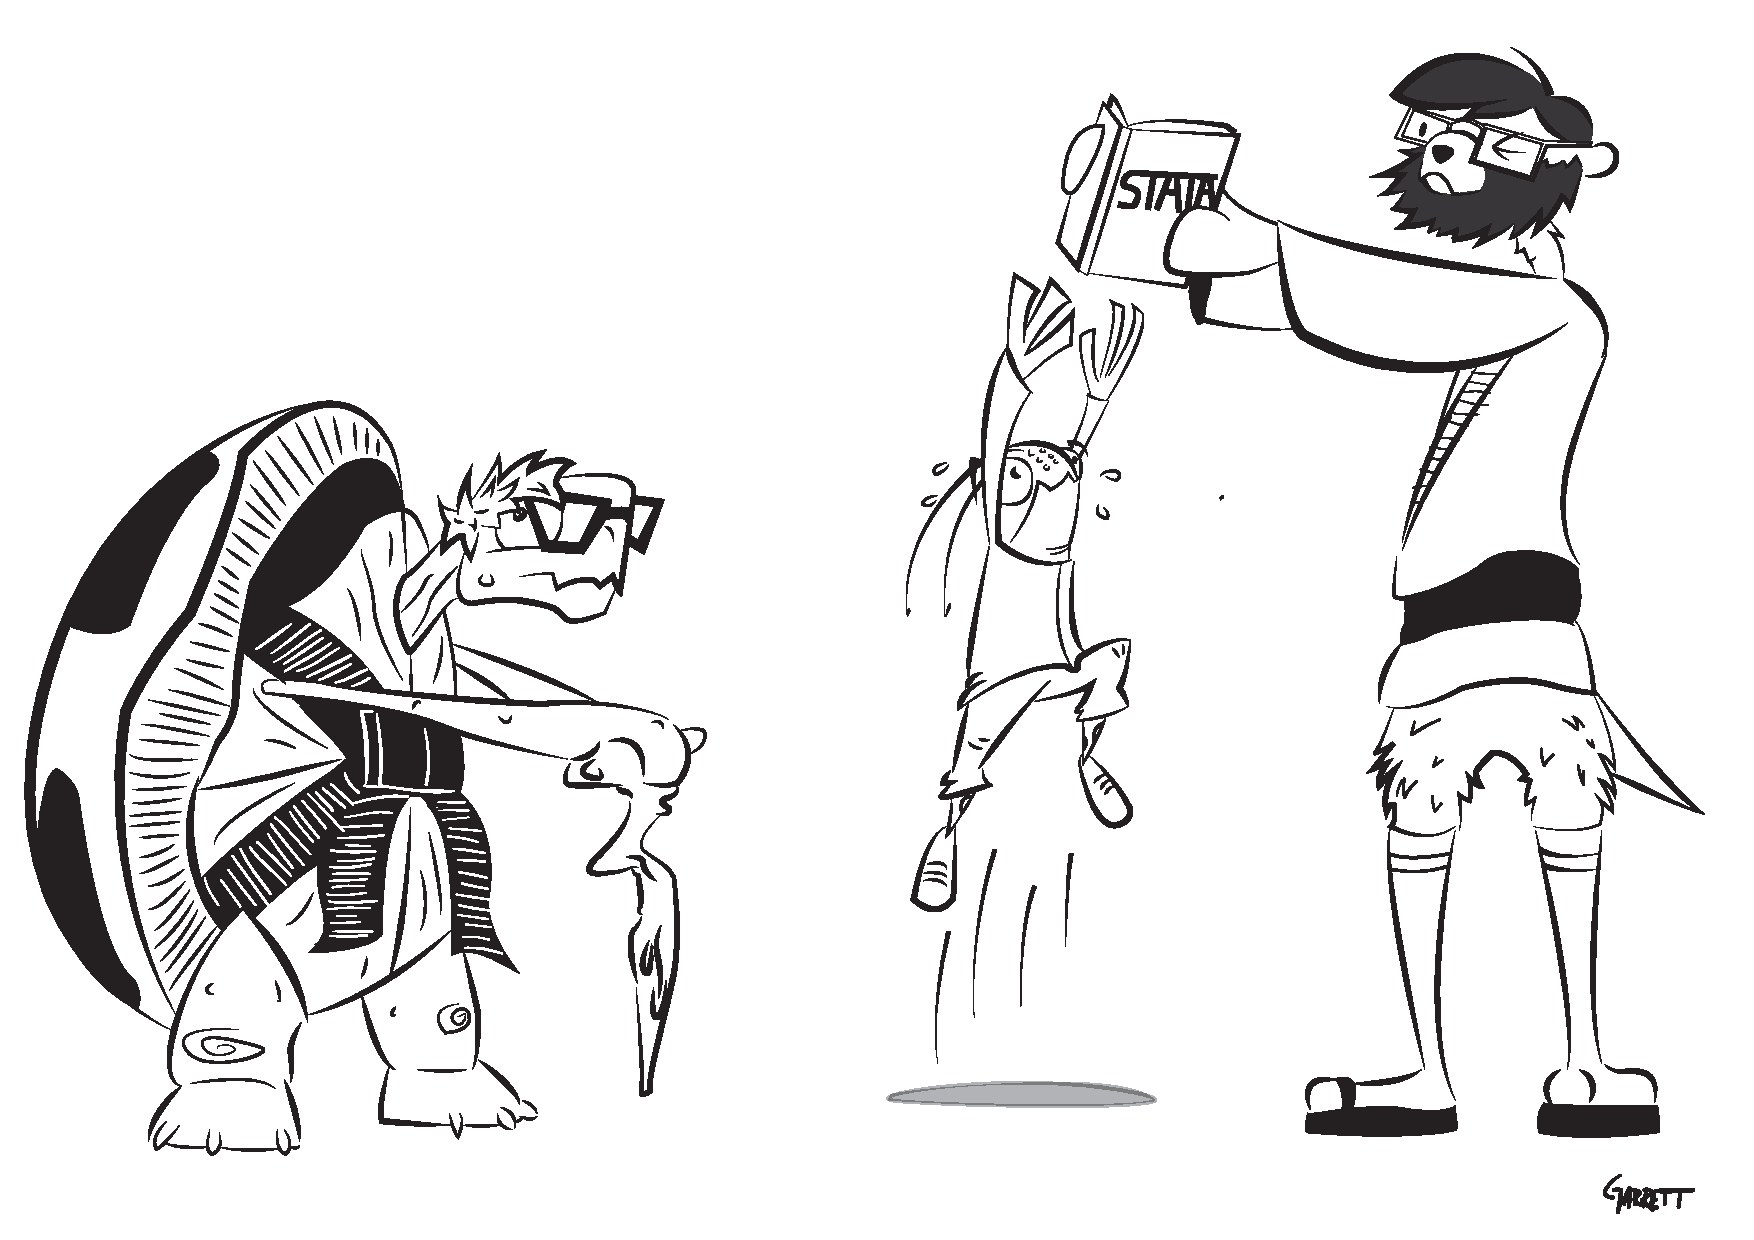
\includegraphics[width=0.57\textwidth]{fig/fig1.pdf}
		\end{center}
	\end{center}
\end{frame}
%==============================================================
% END
%==============================================================
\miniframesoff 	
\begin{frame}[plain, standout]
Gracias! 
\end{frame}

\end{document}		
